\chapter{Implementación}

\noindent

En este capítulo se describe la implementación del sistema basada en el diseño
previamente establecido. Primero se discute la biblioteca de MCTS: mctspy.
Posteriormente, se muestra la clase que implementa las reglas del juego de
dominó y su integración con la biblioteca. Por último, se comenta la integración
del módulo de muestreo con la búsqueda en árbol.

\section{Biblioteca de \textit{Monte Carlo Tree Search}}

Una parte central del sistema es el algoritmo MCTS. Después de buscar distintas
opciones en el Índice de Paquetes de Python (PyPI por sus siglas en inglés) se
decidió utilizar la biblioteca mctspy de Kamil Czarnogórski(2018a). El paquete
se encuentra publicado como código abierto en Github bajo la licencia MIT.

El repositorio cuenta con escasa documentación, pero el estilo de programación
es claro y sencillo, lo que facilita la lectura del código fuente. Para poder
utilizar mctspy para un juego en particular es necesario implementar una clase
que represente el estado del juego, así como los métodos que requiere el
algoritmo. El repositorio cuenta con un ejemplo de implementación para el juego
de gato a partir del cual se puede identificar la interfaz que debe satisfacer
el estado del juego.

Una vez que se ha implementado la interfaz se puede construir un objeto
MonteCarloTreeSearch con el cual se puede invocar la ejecución de MCTS. La clase
requiere un parámetro que determina el número de iteraciones de MCTS que se
ejecutarán. Para facilitar el control sobre el tiempo total de ejecución, se
realizó una contribución a mctspy en la cual se añadió la opción de configurar
el algoritmo con un presupuesto de tiempo. Así, se corren tantas iteraciones
MCTS como se puedan en el lapso establecido.

\section{Implementación de la clase de juego}

Las reglas del juego se implementaron dentro de la clase que representa el
estado del juego. La interfaz que dicha clase debe satisfacer consiste en los
siguientes métodos:

\begin{itemize}
   \item game\_result
   \item is\_game\_over
   \item is\_move\_legal
   \item move
   \item get\_legal\_actions
\end{itemize}

Las manos de los jugadores se modelaron como una lista de conjuntos. Cada ficha
es representada como un conjunto de dos números que corresponden a los puntos de
la pieza. Así, la clase cuenta con los métodos necesarios para transformar el
estado del juego de forma consistente con las reglas del dominó.

\section{Módulo de muestreo}

Por último, se implementó un algoritmo para generar las posibles formas de
repartir las fichas que no se conocen.

\begin{figure}[ht]
   \begin{center}
      \hbox{\hspace{-1.5em} 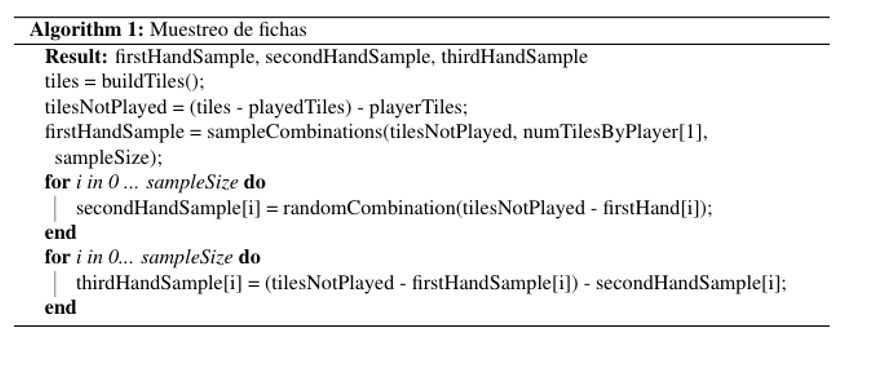
\includegraphics[scale=0.9]{codigo_muestreo.png}}
      \caption{Algoritmo de muestreo. Se generan un conjunto de escenarios consistentes con las fichas observadas}
      \label{CM}
   \end{center}
\end{figure}

Como se muestra en el pseudocódigo de la figura \ref{CM}, primero se generan
todas las fichas del juego (\textit{tiles} en ingles). Luego, se calculan las
fichas que aun no se han jugado (\textit{tilesNotPlayed}) sustrayendo de
\textit{tiles} las fichas que ya se tiraron (\textit{playedTiles}) y las fichas
asignadas al bot (\textit{playerTiles}). Las operaciones de resta corresponden a
la resta de conjuntos, como se utiliza en el lenguaje Python. Posteriormente se
genera el arreglo \textit{firstHandSample}, que contiene las fichas del primer
jugador a la derecha para distintas reparticiones. Se generan la cantidad de
reparticiones definidas en \textit{sampleSize}. Por último, se generan los
arreglos de fichas para el segundo y tercer jugador removiendo las fichas de las
manos de los demás jugadores.

% \noindent El Grupo Huatusco se ha reunido por más de quince años intentando responder la pregunta de por qué México no crece a mayores tasas.

% \begin{figure}[H]
% \begin{center}
% \caption{Brecha entre productividad y remuneración laboral en el mundo (1948-2016)}
% \label{PROD_W}
% \begin{tikzpicture}
% \begin{axis}[
%     xlabel={Año},
%     ylabel={Cambio porcentual acumulado},
%     xtick pos=left,
%     ytick pos=left,
%     xtick={1950,1970,1990,2010},
%     ytick={0,125,250},
%     scale only axis=true,
%     width=0.6\textwidth,
%     height=0.4\textwidth,
% ]

% \addplot[
%     color=red,
%     ]
%     coordinates {(1948,0)
% (1949,1.5)
% (1950,9.3)
% (1951,12.4)
% (1952,15.6)
% (1953,19.5)
% (1954,21.6)
% (1955,26.5)
% (1956,26.7)
% (1957,30.1)
% (1958,32.8)
% (1959,37.6)
% (1960,40)
% (1961,44.4)
% (1962,49.8)
% (1963,55)
% (1964,60)
% (1965,64.9)
% (1966,70)
% (1967,72.1)
% (1968,77.2)
% (1969,77.9)
% (1970,80.4)
% (1971,87.1)
% (1972,92)
% (1973,96.7)
% (1974,93.7)
% (1975,97.9)
% (1976,103.4)
% (1977,105.8)
% (1978,107.8)
% (1979,108.1)
% (1980,106.6)
% (1981,111)
% (1982,107.9)
% (1983,114.1)
% (1984,119.7)
% (1985,123.4)
% (1986,128)
% (1987,129.1)
% (1988,131.8)
% (1989,133.7)
% (1990,137)
% (1991,138.9)
% (1992,147.6)
% (1993,148.4)
% (1994,150.7)
% (1995,150.9)
% (1996,156.9)
% (1997,160.5)
% (1998,165.7)
% (1999,172.1)
% (2000,178.5)
% (2001,182.8)
% (2002,190.7)
% (2003,200.2)
% (2004,208.2)
% (2005,213.6)
% (2006,215.5)
% (2007,217.7)
% (2008,218.2)
% (2009,224.7)
% (2010,234.3)
% (2011,234.7)
% (2012,236.5)
% (2013,237.6)
% (2014,239.3)
% (2015,241.1)
% (2016,241.8)
%     };

%     \addplot[
%     dashed,
%     color=blue,
%     ]
%     coordinates {(1948,0)
% (1949,6.3)
% (1950,10.5)
% (1951,11.8)
% (1952,15)
% (1953,20.8)
% (1954,23.5)
% (1955,28.7)
% (1956,33.9)
% (1957,37.1)
% (1958,38.2)
% (1959,42.6)
% (1960,45.5)
% (1961,48)
% (1962,52.5)
% (1963,55)
% (1964,58.5)
% (1965,62.5)
% (1966,64.9)
% (1967,66.9)
% (1968,70.7)
% (1969,74.7)
% (1970,76.6)
% (1971,82)
% (1972,91.3)
% (1973,91.3)
% (1974,87)
% (1975,86.9)
% (1976,89.7)
% (1977,93.1)
% (1978,96)
% (1979,93.5)
% (1980,88.6)
% (1981,87.6)
% (1982,87.8)
% (1983,88.4)
% (1984,87)
% (1985,86.3)
% (1986,87.3)
% (1987,84.6)
% (1988,83.9)
% (1989,83.7)
% (1990,82.2)
% (1991,81.9)
% (1992,83.1)
% (1993,83.4)
% (1994,83.8)
% (1995,82.7)
% (1996,82.8)
% (1997,84.8)
% (1998,89.2)
% (1999,91.9)
% (2000,92.9)
% (2001,95.6)
% (2002,99.4)
% (2003,101.7)
% (2004,100.9)
% (2005,100.1)
% (2006,100.2)
% (2007,101.7)
% (2008,101.7)
% (2009,109.7)
% (2010,111.6)
% (2011,109.1)
% (2012,107.3)
% (2013,108.3)
% (2014,109.2)
% (2015,112.8)
% (2016,115.1)};

% \end{axis}
% \end{tikzpicture}

% \imagesource{elaboración propia con datos del Economic Policy Institute.}
% \end{center}
% \end{figure}

% % Gráfica con dos colores a mano
